%!TeX spellcheck = de_DE
%\documentclass[a4paper,cleardoubleempty,BCOR1cm]{scrbook}
\documentclass[a4paper,cleardoubleempty,BCOR1cm]{book}

% use to waste space:
% \documentclass[12pt,a4paper]{article}

% if you have this style and like it.
%\documentclass{acmsiggraph}
%\documentclass[review]{acmsiggraph}      % review
%\documentclass[widereview]{acmsiggraph}  % wide-spaced review
%\documentclass[preprint]{acmsiggraph}    % preprint

% define a \comment{this is a comment which can have linebreaks in it}
\newcommand{\comment}[1]{}
% \newcommand{\todo}[1]{\marginpar{\bf{#1}}}
\newcommand{\todo}[1]{{\color{red}\bf{TODO: #1}}}

\usepackage{mathptmx}
\usepackage[pdftex]{graphicx}
\usepackage[pdftex]{color}
\definecolor{rot}{RGB}{165,30,55} %rote Farbe
\graphicspath{{./images/}}
\usepackage{parskip}
\usepackage{amsmath}
\usepackage{dsfont}
\usepackage{pxfonts}

\usepackage[T1]{fontenc}
\usepackage{textcomp}

% comment these two lines out if you don't want minion/myriad fonts.
% \usepackage[minionint,mathlf]{MinionPro}
% \renewcommand{\sfdefault}{Myriad-LF}
%\usepackage{Myriad}

% no page number on float pages, fixes problems with overlarge diagrams.
\usepackage{fancyhdr}
\pagestyle{fancy}
%\lhead{}
%\chead{}
%\rhead{}
%\lfoot{}
\fancyhf{}
\fancyhead[EL]{\nouppercase{\leftmark}}
\fancyhead[OR]{\nouppercase{\rightmark}}
\cfoot{}
%\fancyfoot[EL]{\iffloatpage{}{\thepage}}
%\fancyfoot[OR]{\iffloatpage{}{\thepage}}
\fancyfoot[EL]{\thepage}
\fancyfoot[OR]{\thepage}
\renewcommand{\headrulewidth}{0pt}
\renewcommand{\footrulewidth}{0pt}

%\usepackage{natbib}		% textual referencing
%\usepackage[numbers,super]{natbib}	% nice superscripts
%\bibliographystyle{chicago}	% shitty
\bibliographystyle{alpha}	% abbr names and year in \cite
%\bibliographystyle{agsm}	% australian, need natbib
%\bibliographystyle{kluwer}	% need natbib
%\bibliographystyle{apalike}	% lengthly
%\bibliographystyle{abbrv}	% minimal?

% use for german line breaking:
%\usepackage[ngerman]{babel}
\usepackage[T1]{fontenc}
\usepackage[utf8x]{inputenc}

% avoid us-style text color destruction:
\frenchspacing
\usepackage{microtype}

% have a nice framebox with border directly around the image:
\fboxsep 0pt
\newcommand{\fimg}[2]{\fbox{\includegraphics[width=#1]{#2}}}

\usepackage{theorem}
\theorembodyfont{\upshape}
\newtheorem{definition}{Definition}

\usepackage{listings}
\lstset{numbers=left, numberstyle=\tiny, basicstyle=\tiny, language=C++}
\usepackage[boxruled]{algorithm2e}
%\usepackage{hyperref}
\usepackage{url}
\usepackage{subfig}

\def\code#1{{\tt{#1}}}



\usepackage[main=ngerman]{babel}

\pagenumbering{roman}
\title{Thesis Template}
\author{Tolga Demir \thanks{e-mail: tolga.demir@student.uni-tuebingen.de}}
\date{\today}
\begin{document}

\begin{tabular}{lr}
% 
\includegraphics[width=0.5\linewidth]{logo_sw} % logo bw
 
\includegraphics[width=0.5\linewidth]{UT_WBMW_Rot_4C} % logo red
 & \hspace{0.2\linewidth}
 \parbox{0.5\linewidth}{
   \large\bf\textsf{\color{rot}{Mathematisch-\\Naturwissenschaftliche\\Fakultät\\\\}}
  \hspace{-.144cm}\normalsize\textsf{\color{rot}{Kognitive Systeme}}
   \vspace{0.6cm}
 }
\end{tabular}

\vspace*{10ex}
Bachelorarbeit

{\huge\bf\textsf{Modernisierung des CT'Bot und Implementierung eines SLAM-Framework in Python}}

\vspace*{30ex}

Eberhard Karls Universität Tübingen\\
Mathematisch-Naturwissenschaftliche Fakultät\\
Wilhelm-Schickard-Institut für Informatik\\
Kognitive Systeme\\
Tolga Demir,~ \verb+tolga.demir@student.uni-tuebingen.de+,~ 2019

\vspace*{5ex}

\begin{tabular}{@{}l@{\hspace{2em}}l}
  Bearbeitungszeitraum:& 01.04.-31.07.2019 \vspace*{5ex} \\
  Betreuer/Gutachter:& Prof. Dr. Andreas Zell, Universität Tübingen\\
\end{tabular}

\thispagestyle{empty}
\newpage

\chapter*{Selbstst\"andigkeitserkl\"arung}
Hiermit versichere ich, dass ich die vorliegende Bachelorarbeit selbst\"andig und
nur mit den angegebenen Hilfsmitteln angefertigt habe und dass alle Stellen,
die dem Wortlaut oder dem Sinne nach anderen Werken entnommen sind,
durch Angaben von Quellen als Entlehnung kenntlich gemacht worden sind.
Diese Bachelorarbeit wurde in gleicher oder \"ahnlicher Form in keinem anderen
Studiengang als Pr\"ufungsleistung vorgelegt.

\vspace*{8ex}
\hrule
\vspace*{2ex}
Tolga Demir (Matrikelnummer 123456), \today


\chapter*{Abstract}




\chapter*{Acknowledgments}
Mein Dank gilt Prof. Zell, der diese Bachelorarbeit engagiert begleitet und ermöglicht hat. \\
Weiterhin möchte ich mich herzlich beim Wohnheim Rechberghaus bedanken für die Bereitstellung einer Werkstatt. Ohne diese Hilfe wären mir manche Arbeiten am Roboter kaum möglich gewesen. 

\tableofcontents

\clearpage
\pagenumbering{arabic}

\chapter{Einführung}

% ganze Kapitel 5 Seiten max
\section{Autonome Mobile Roboter}
Mobile Roboter werden für eine breite Bandbreite an Arbeiten eingesetzt, darunter die Erkundung von menschenfeindlichen Umgebungen, das Verrichten von Arbeiten in diesen oder als Service-Roboter z.B. zum Rasenmähen oder Staubsaugen.\\
Die Bezeichnung autonom meint hierbei, dass die Roboter ihre Aufgaben (fast-) selbstständig erledigen. Dazu gehören neben der reinen Tätigkeit auch Themen wie das Fahren, Erfassen von Zielen, Erstellen von Karten ihrer Umgebung und zurecht finden in unbekanntem Terrain. \\
Mobile Roboter sind seit den 1960ern ein Feld intensiver Forschung mit vielen Applikationen in der Industrie. Seit den 2000ern werden eine Vielzahl von verschiedenen Mobilen Robotern für die Industrie verkauft. Diese frühen Generationen von Robotern sind aus heutiger Sicht überholt. Oft lässt sich weder die Hardware noch die Software für moderne Anforderungen konfigurieren.\\
Eine Kernfrage dieser Arbeit ist, ob sich ein solcher Roboter, exakter: der Ct'Bot des Heise Verlags aus dem Jahr 2006 mit minimalem Aufwand in Kosten und Umbau so neu gestalten lässt, dass er diesen Herausforderungen gewachsen ist. \\
Dies würde die Wiederverwertbarkeit älterer Roboter ermöglichen und so einen erheblichen Beitrag zu Kostensenkung und Umweltschutz garantieren, welche mit einer Neuanschaffung nicht zu realisieren wären. 

\section{Ziel dieser Arbeit}
Diese Bachelor-Arbeit widmet sich der Erneuerung des Ct'Bots. Dieser soll von Grund auf modernisiert und fit gemacht werden für die Anforderung neuerer Algorithmen und Datenschnittstellen. Der Roboter soll dabei nicht an Größe gewinnen und seine Vorteile weiterhin behalten. \\

Zugleich wird ein Python Framework entwickelt, welches ein solides Gerüst für weitere Anwendungsentwicklungen darstellt. Es soll intuitiv und schnell einsetzbar sein und die komplette Funktionalität des Roboters bereitstellen. Hierdurch wird dem Roboter ein neuer Einsatzzweck ermöglicht. \\


\section{Methodik und Beschränkungen}

Durch Analyse der vorhandenen Hardware sollen Lücken im Funktionsumfang ausgebessert und der Roboter befähigt werden, eine moderne SLAM-Implementation (Simultainous Self-Lokalization and Mapping) autonom auszuführen. 
Dabei müssen die beschränkte Genauigkeit kostengünstiger Sensorik beachtet werden. Weiterhin soll die Modernisierung ein Budget von 100Euro für neue Hardware nicht übersteigen. 

\section{Gliederung und Aufbau}

Diese Arbeit erörtert im Folgenden die Grundlagen der Mobilen Robotik Hardware und- eingeschränkt- das Thema SLAM. Danach wird ausführlich über die vorhandene Hardware und die Erneuerung des Roboters berichtet. Für den fertigen Roboter wird dann ein Software-Framework vorgestellt, welches eine Plattform für die komplette Funktionalität darstellt. \\
Abschließend werden verschiedene  Tests des Prototypen präsentiert und die Ergebnisse erörtert. \\
Mit einer Zusammenfassung der Arbeit und einen Ausblick endet diese Dokumentation.  





% ganze Kapitel 5 Seiten max
\chapter{Grundlagen}
In diesem Kapitel werden die Grundlagen, welche zum Verständnis dieser Arbeit benötigt werden kurz erläutert.

\section{Hardware Mobiler Roboter}
Ein Mobiler Roboter besteht aus mindestens einer Hauptplatine für die Steuerung, einer Möglichkeit der Fortbewegung und einer Energie-Quelle. \\


\section{Mobile Hardware und ihre Lebenszeit}
Gordon Moore behauptete 1965, dass sich die Komplexität von Integrierten Schaltkreisen alle zwei Jahre verdoppeln würde \footnote{ G. E. Moore: Cramming more components onto integrated circuits. In: Electronics. Band 38, Nr. 8, 1965, S. 114–117}. Diese Aussage wurde bekannt als das Mooresche Gesetz und hält sich bis heute. Die Konsequenz daraus ist, dass jeder neu entwickelte Chip innerhalb weniger Jahre als Leistungsschwach gilt und nicht mehr dem Stand der Technik entspricht. Eine derart radikale und dauerhafte Erneuerung kennt sonst kein Industrieprodukt. Diese schnelllebige Entwicklung setzt sich vom Chip fort auf die fertigen Systeme. Insbesondere Mobile Roboter erleben mit jeder weiteren Generation einen enormen Leistungsschub. Durch die Knappheit von Ressourcen die eine Mobile Hardware mit sich bringt fällt jede weitere technische Innovation schwerer ins Gewicht. Sinkt zum Beispiel der Stromverbrauch des Hauptprozessors, so steigt als Folge die Laufzeit des akku-betriebenen Mobilen Roboters, während dieser Aspekt bei standort-gebundener Hardware kaum Nutzen bringt. Sinkt das Gewicht und die Größe von Sensorbauteilen so wirkt sich das ebenso erheblich auf Erscheinung, Funktionsumfang und -dauer des Mobilen Roboters aus. Welche Auswirkungen diese Entwicklungen hat lässt sich sehr anschaulich am Roboterhersteller Boston Dynamics beobachten. Ihr 4-Beiniger Roboter BigDog wurde 2009 vorgestellt und sollte ein Mobiler Roboter zum Transport von schweren Gewichten in Wald- und Landwirtschaftsgebieten sein. Es war ihm dabei schon möglich seine Balance - auch gegen Widerstand - zu halten und geführte Wege abzuschreiten. Vergleicht man ihn jedoch mit dem 2017 vorgestellten SpotMini, so erkennt man den enormen Sprung der Technik. So erreicht der neue SpotMini Laufgeschwindigkeiten von über 100 Km/H und hat eine Last-Laufzeit welche ein Vielfaches seines Vorgängers ist. \\
Die Konsequenz dieser Erkenntnis wäre, Hardware und jede Chip-gebundene Technik im 2-3 Jahres-Rythmus zu tauschen. Betrachtet man bei dieser Überlegung jedoch die Wirtschaftlichen und Umweltpolitischen Aspekte, so scheint das kontraproduktiv. Moderne Roboter können Preise bis weit über einen 6-stelligen Euro Betrag kosten (z.B betragen die reinen Produktions- und Entwicklungskosten des Atlas2 1 Mio Dollar pro Stück). Versucht man nun seine Wirtschaftlichkeit auf einer Einsatzdauer von 2 Jahren zu brechnen, so muss das Resultat negativ ausfallen. \\
Gerade in Unternehmen, wird Hardware daher oft so lange wie möglich genutzt. Zumindest solange eine Möglichkeit besteht diese an die geforderten Arbeitsprozesse anzupassen. \\

Innerhalb der Sensorik-Komponenten ist die Entwicklung ähnlich gelagert - wenn auch die Erneuerung nicht so schnell wie im Chip-Bereich ausfällt. Insbesondere sind viele Sensoren früh in ihrer heute üblichen Form auf den Markt gekommen. Das zeigt z.B. der Reflexoptokopter wie er auch in unserem Roboter verbaut ist. Der CNY70 ist in seiner jetzigen Bauform schon seit 2001 auf dem Markt. Seitdem hat sich zwar der preis radikal reduziert (von einem hochklassigen Sensor zu einem 1Cent Produkt), jedoch nicht seine Einsatzgebiete. Reine Sensor-Produkte sind somit mehr von ihrer internen Laufzeit abhängig als von der Entwicklung des Marktes. Da sie sehr häufig für einen spezifischen Zweck gebraucht werden und keine frei programmierbaren Teile sind. 


\section{Software Mobile Roboter}
Moderne Mobile Roboter haben meist ein eigenes Betriebssystem, welches ihre Funktionen im Ganzen steuert und dem Anwender die Funktionalität als (modulares-) Framework bereitstellt. Dies erlaubt es Roboter, welche unterschiedlichste Hardware und Sensorik haben, schnell und einfach zu kontrollieren. Hierbei ist vor allem das Robot Operating System (ROS) in der Forschung weit verbreitet. ROS arbeitet mit einem Baukasten-Prinzip, welches über Knoten die Anbindung von Sensoren und ihren Daten an einen Roboter erlaubt. Roboterhersteller entwickeln hierauf aufbauend eigene Betriebssysteme oder Frameworks. So nutz reines ROS z.B. ABB. Während KUKA ihr selbst entwickeltes KRL einsetzt. Ebenso Fanuc mit Karel. \\
ROS, als open-source Projekt, wird von den Nutzern ständig weiterentwickelt und um Funktionalitäten erweitert. So sind komplexeste Algorithmen und Sensorsteuerungen direkt im System vorhanden und müssen nicht jedes Mal neu gedacht werden. Dies ist als seine größte Stärke zu betrachten. Von Nachteil ist die Komplexität des Systems. Die vorhandenen Möglichkeiten zur Sensoranbindung und Algorithmen-Steuerung machen ROS unübersichtlich und führen zu vielen Fehlern bei weniger geüübten Nutzern. Weiterhin ist ROS ein großes System. Viele ältere Roboter und schwächere Hauptprozessoren sind nicht in der Lage ROS als Ganzes zu hosten. Zudem kann ROS Die Kanone sein, mit der auf Spatzen geschossen wird. Nicht jeder Mobile Roboter braucht das vollständige ROS, oft sind diese mit einem kleinen, für sie geschriebenen System schneller und zuverlässiger. \\
Als Alternativen für kleinere Systeme haben sich Rasbian, Embedded Linux oder Windows CE etabliert. Die Wahl hängt hier vom Hauptprozessor oder der Steuerungseinheit ab. So eignet sich der Rasbian dann, wenn der Mobile Roboter von einer Raspberry Pi gesteuert wird. Während Arduino eine einfache Möglichkeit ist C Code auf einem gleichnamigen Chipset zu implementieren. Windows CE ist eine verschlankte Windows-Variante und sollte zu Beginn ein Betriebsystem für Mobilen Roboter darstellen. Es entwickelte sich aber eher in Richtung Mobile Telefone und Konsumenten-Endgeräte und wird daher kaum noch im Roboter bereich genutzt. \\
Zu diesen Betriebssystemen gibt es noch weitere, spezialisierte Echt-Zeit-Betriebssysteme wie RTLinux oder VxWorks. Diese werden für die Controlle und Vernetzung einzelner Hardware-Komponenten genutzt. Seltener als Framework oder Betriebssystem für einen kompletten Roboter. \\

Die wichtigsten Eigenschaften eines Roboter-Frameworks sind somit :
\begin{itemize}
	\item Wenig Speicherverbrauch:\\
			Durch die Begrenzung des Speicherplatzes vieler Mobiler Roboter ist ein kleines Betriebssystem zu bevorzugen. 
	\item Schnelligkeit und Möglichkeit der Echt-Zeit-Datenverarbeitung: \\
			Hier müssen insbesondere Sensorik-Messdaten direkt ausgelesen und verarbeitet werden können. Dies muss schnell passieren. So braucht z.B. ein klassischer Ultraschall-Sensor für den Betrieb mind. eine Verbindung zum Verarbeitenden System, welche in Schallgeschwindigkeit die Messdaten ablesen kann. 
	\item Geringer Energieverbrauch:\\
			Im Bereich der Mobilen Roboter dient der Akku als Hauptstromquelle. Dieser begrenzt die Laufzeit des Systems. Umso weniger der Roboter im Ruhezustand verbraucht umso länger kann er agieren. 
	\item Möglichkeit der Sensor-Angliederung:\\
			Das Betriebsystem muss befähigt sein Sensoren anzusprechen und Daten von diesen Empfangen zu können.
\end{itemize}

Klassische Merkmale moderner Betriebssysteme, wie ein User-Interface, Daten-Manager oder Ausführbarkeit von 3D-Visualisierungen sind in der Robotik kein Thema. 

\section{SLAM - Simultainous Self-Lokalization and Mapping }
Die Grundlage der jeder Interaktion mit seiner Umwelt stellt beim Mobilen Roboter seine Karte dar. Der Roboter bewegt sich innerhalb seiner Umwelt und muss dabei jederzeit wissen wo er sich befindet und wie er zu einem Bezugspunkt ausgerichtet ist. \\
Mit Hilfe seiner Karte und seiner Ausrichtung kann nun der Roboter sich in seiner Umwelt bewegen, bestimmte Ziele ansteuern und Aufgaben erledigen. Startet der Roboter in einem unbekannten Umfeld, so muss er diese Karte selbstständig generieren. Dieser Prozess wird als SLAM bezeichnet. Dabei erkundet der Roboter den Raum, erfasst die wichtigsten Umwelt-Daten und hält seine veränderte Position zu jedem Zeitpunkt fest. \\
Dies wird häufig als Henne-Ei-Problem bezeichnet, da der Roboter weder die Umgebung kennt noch seine Position in dieser und trotzdem beide Parameter schätzend berechnen muss. \\
Ermöglicht wird ein SLAM- Algorithmus durch die Sensorik des Roboters. Dazu braucht er -meist - zwei Dinge: 
\begin{enumerate}
	\item Odometrie:\\
	 Er muss jede Änderung seiner Position und Ausrichtung exakt messen können. Kann er dies nicht, so verliert er seine Position im Verhältnis zum Ausgangspunkt und die Karte kann nicht mehr korrekt berechnet werden. Dies nennt man Odometrie. In den frühen Jahren wurden hierfür Radsensoren eingesetzt. Diese sollten jede Bewegung des Roboterrads messen und damit Rückschlüsse auf gefahrene Strecke und Ausrichtung erlauben. Dies lässt sich einfach implementieren, gilt jedoch aufgrund von "wheel slips" (Radbewegungen ohne Bewegungen des Roboters oder Bewegung des Roboters ohne Bewegung der Räder) als sehr ungenau. \\
	 Eine weitere Möglichkeit stellen Optical-Flow-Sensoren dar. Diese nehmen aus kürzester Distanz Bilder des Bodens auf. Jede Bewegung des Roboters resultiert nun in einer Verschiebung innerhalb des Bildes. Diese kann berechnet werden und gibt die Veränderung zwischen jeder Bewegung exakt wieder. Optical-Flow-Sensoren werden z.B. in Computer-Mäusen eingesetzt. In der Robotik sind Sie eine Nische, da ihre Nachteile (Sensor muss nah am Boden verbaut sein, Untergrund muss glatt und sauber sein) überwiegen. \\
	 Odometrie Daten können auch über Kameras gewonnen werden. Diese funktionieren wie ein Opti-Flow-Sensor auf einem hoch-frequentierten Vergleich der Bilder miteinander. \\
	 Ebenso eignen sich hierzu Lidar-Sensoren. Diese werden in neuesten Robotern standartmäßig genutzt. Ihre Messungen sind die Exaktesten, jedoch brauchen Sie komplexere Algorithmen und - ihr größter Nachteil - sind vergleichsweise teuer. Dafür erlauben Sie, ebenso wie manche Kameras, die implementierung von Algorithmen, welche Odometrie und Distanzmessung vereinigen. 
	\item Sensorik um Distanzen zu messen. Bewegt sich der Roboter, muss er erkennen wo Hindernisse sind. Dies wird durch Distanz-Sensoren erreicht. Der Roboter misst nach jeder Bewegung die Abstände um ihn herum und kann so erkennen wie die Karte zu gestalten ist. 
\end{enumerate}

Mit diesen gewohnnen Daten kann der SLAM-Algorithmus eine Karte entwickeln. Algorithmen wie der Kalman-Filter vereinigen dabei beide Punkte - Odometrie und Distanzmessung- in Einem. Viel genutze Methoden sind beispielhaft PartikelFilter, Kalman-Filter oder Graphen-basierte SLAMs. Alle Algorithmen haben dabei besondere Voraussetzungen an die genutzte Sensorik und die Genauigkeit der Daten. 


\section{Zusammenfassung}
Hard- und Software bilden gemeinsam den Kern dieser Arbeit. Wie veranschaulicht wurde, braucht der Ct'Bot für versch. Aufgabenstellungen eine Möglichkeit sich in der Welt zurecht zu finden und sich ein Bild von dieser machen zu können. Im folgenden Kapitel soll mit Hilfe dieses theoretischen Wissens der vorhandene Roboter analysiert werden und jede seiner Komponenten auf Funktionsfähigkeit untersucht werden. \\
Danach wird die Software betrachtet und Entscheidungen bezüglich Umfang und Auswahlkriterien getroffen. 









% ganze Kapitel 10 Seiten max
\chapter{Ct'Bot}
Der Ct'Bot wurde 2006 von der Zeitschrift Ct' des Heise Verlags herausgebracht. Er kostete in der Basisversion ab 250Euro und kam als Baukasten. Die Bauteile wurden halb-fertig geliefert. Der Kunde musste versch. Bauteile auf die Platinen löten und das Ganze zusammenschrauben. \\
Der fertiggestellte Roboter ließ sich über ein mitgeliefertes Kabel an den PC anschließen und programmieren. Kern der Software bildete ein offenes Betriebssystem, welches extra für den CT'Bot geschrieben war. Die Kern-Software war dabei gestellt und wurde durch User ständig erweitert. So wuchs die Kern-Bibliothek an Funktionen mit der Anzahl der Nutzer. \\
Die Software selbst war in der Programmiersprache C gehalten und besaß weiterhin eine Simulationsumgebung, welche geschriebenen Code in einer virtuellen Welt testen konnte. \\
Leider ist das Projekt inzwischen eingestellt und wird nicht mehr vom Produzenten unterstützt. Es gibt keinen Zugriff mehr auf die Programmier-Bibliotheken und Ersatzteile können nicht mehr nachgekauft werden. Ebenso sind alle erschienen Artikel und das CT'Bot-Wikipedia verschwunden oder hinter Bezahlschranken. Das Projekt gilt als ausgestorben. \\
Der Ct'Bot dieser Arbeit wurde im Rahmen einer Doktor-Arbeit aufgebaut. Ziel war ein Multi-Slam-Algorithmus mit mehreren CT'Bots, welche von einem Controll-Tower geleitet wurden. Danach kam er nicht mehr zum Einsatz. 

\section{Erneuerung der Hardware}
In diesem Kapitel wird die vorhandene Hardware analysiert und Verbesserungspotenzial untersucht. Dabei wird abgewogen zwischen jetziger Leistungsfähigkeit und der Möglichkeit neuer Sensorik sowie dem Preis dieser. 

\subsection{Vorhandene Hardware}

\subsubsection{Hauptplatine}

\subsubsection{Wheel-Encoder und Cliff-Detektoren}

\subsubsection{Motor}

\subsubsection{Distanzsensoren}

\subsubsection{Kompass}

\subsubsection{Optical-Flow Sensor}


\subsubsection{LCD}

\subsubsection{Kamera}

\subsubsection{verschiedene Chips}

\subsubsection{Grundplatte}

\subsection{Neue Hardware}

\subsubsection{Hauptplatine}

\subsubsection{Sensorplatine}

\subsubsection{Akku}


\subsubsection{Wheel-Encoder}

\subsubsection{Distanzsensoren}

\subsubsection{Gyroskop}

\subsubsection{LCD}

\subsubsection{Kamera}

\subsubsection{Grundplatte}


% ganze Kapitel 10 Seiten max
\section{Software-Framework}

\subsection{Python}

\subsection{PyBot- Framework}

\subsection{Hardware Treiber}

\subsection{SLAM}



% ganze Kapitel 10 Seiten max
\section{Evaluierung}

\subsection{Testumgebung}

\subsection{Ergebnis}

\subsection{Diskussion und Bewertung}


\subsection{Zusammenfassung}




% 5 Seiten max
\chapter{Zusammenfassung und Ausblick}

\section{Zusammenfassung}

\section{Ausblick}




\section{Literaturverzeichnis}

% ... input content via other .tex files
%\chapter{Conclusion}
\label{sec:conclusion}

To conclude...

\appendix
\chapter{Anhang}
\section{Baupläne}
\subsection{obere Platte}
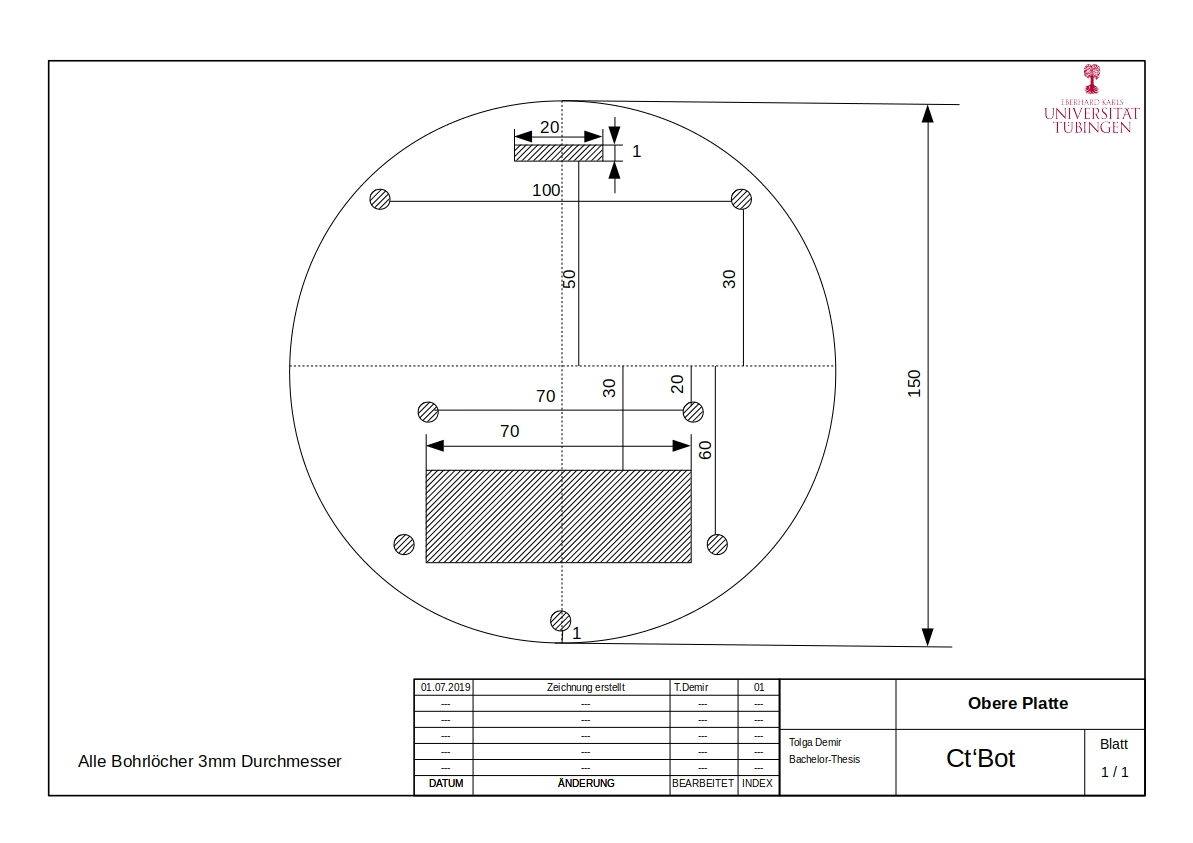
\includegraphics[angle=90,origin=c, scale= 0.5]{images/Zeichnung_obere_Platte.jpg}
\subsection{Mittlere Platte}
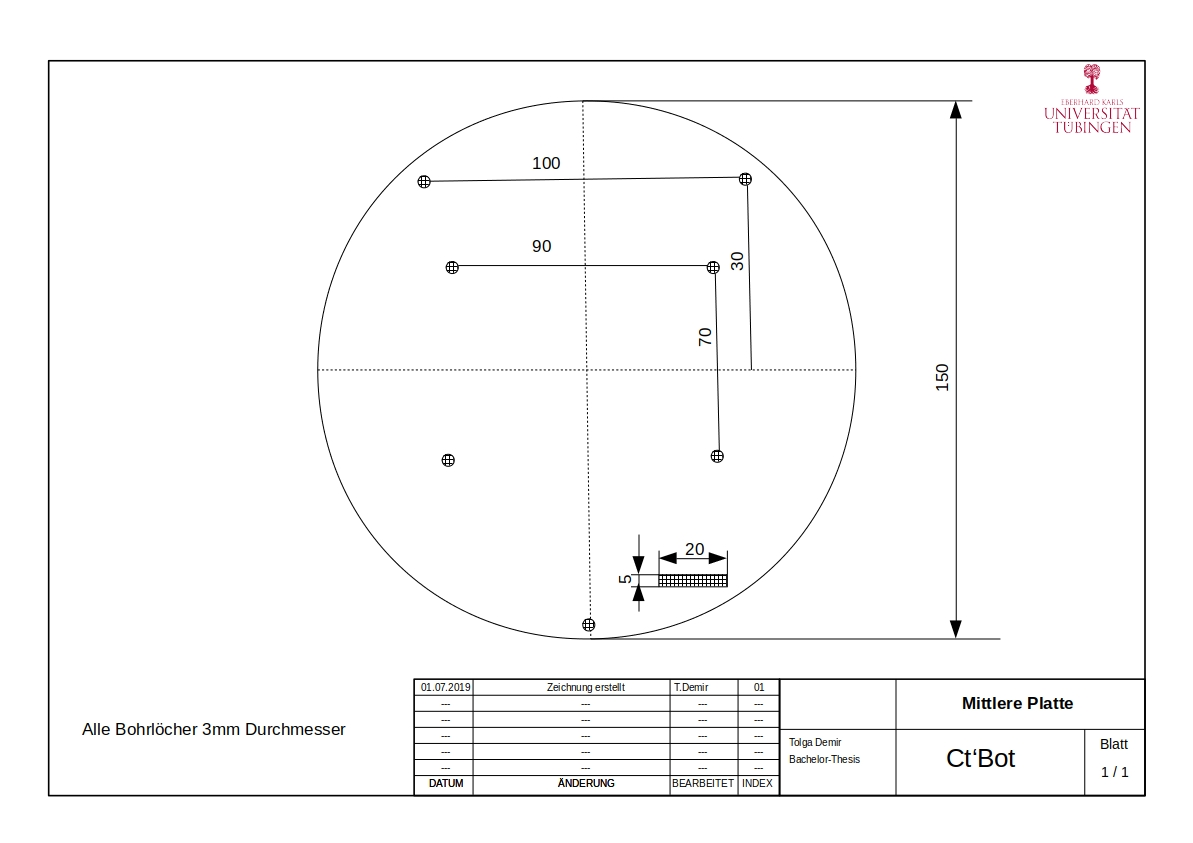
\includegraphics[angle=90,origin=c, scale= 0.7]{images/Zeichnung_mittlere_Platte.jpg}
\subsection{Bodenplatte}
%\includegraphics[angle=90,origin=c, scale= 0.7]{images/Zeichnung_Bodenplatte.jpg}
\subsection{Akku-Träger}
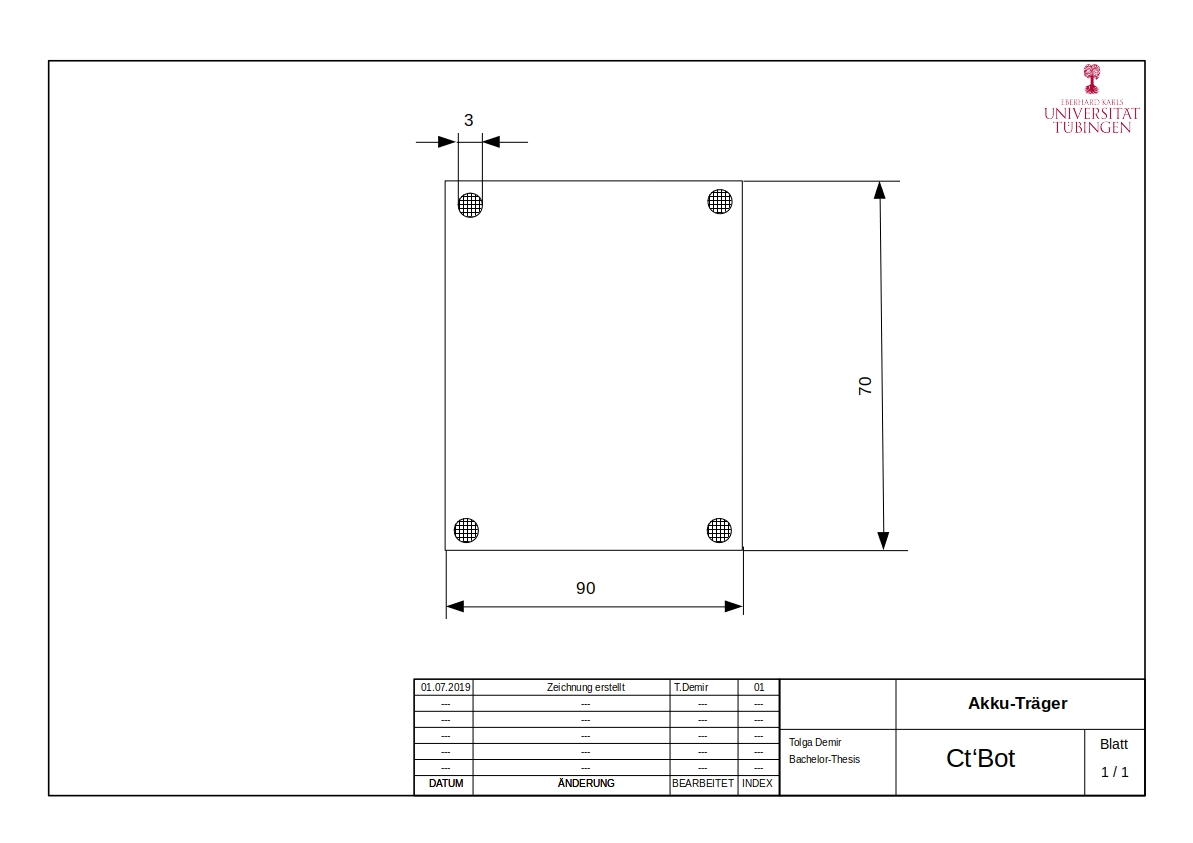
\includegraphics[angle=90,origin=c, scale= 0.7]{images/Zeichnung_Akku.jpg}
\subsection{PCB-Layout}
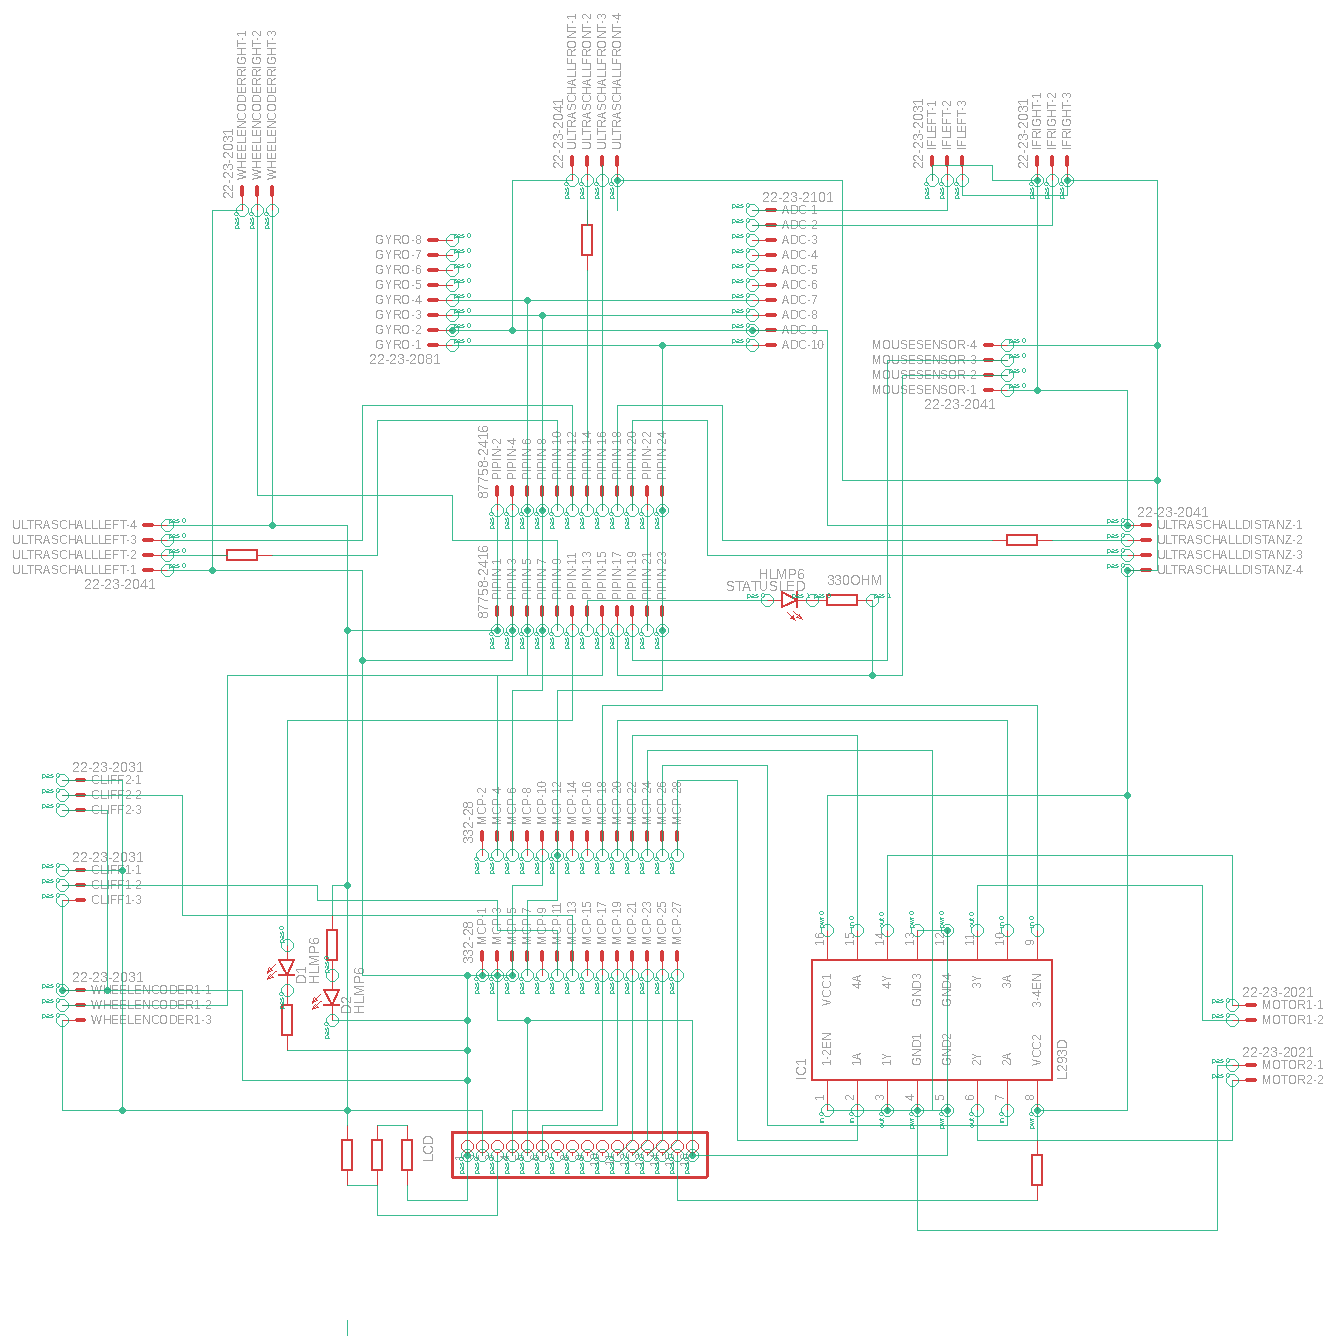
\includegraphics[angle=0,origin=c, scale= 0.75]{images/Layout.png}
\subsection{PCB-Bestückung}
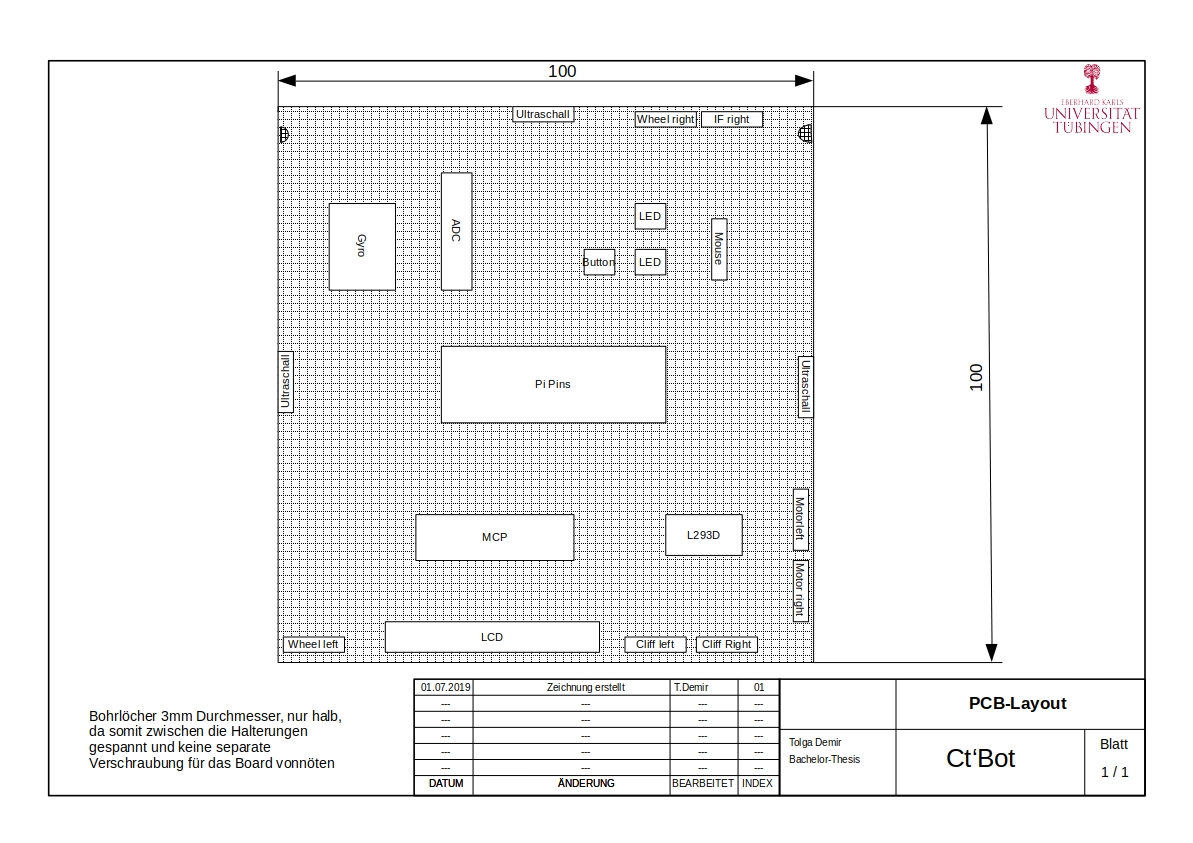
\includegraphics[angle=90,origin=c, scale= 0.7]{images/PCB-Layout.jpg}

\section{Pin-Belegung}
\subsection{Pinbelegung an der Pi}
Die Pinbelegung orientiert sich an der physischen Verteilung der Pins auf der Pi (BCM-Layout). Vorsicht: Hier wird BCM genutzt, die Python Scripts verwenden jedoch BOARD-Layout. \\
Von 24 frei programmierbaren Pins sind 17 in Benutzung, davon 2 für I2C-Kommunikation. 

\begin{center}
	\begin{tabular}{|cc|c|c|}
		\hline
		Pin 	&BCM		& Function 		& Bauteil\\
		\hline
		2		&3			& I2C - SDA		& ADC , Gyro, MCP23017 (daran LCD, Buttons) \\
		3 		&5			& I2C - SCL		& ADC , Gyro, MCP23017 (daran LCD, Buttons)\\
		4		&7			& Freier Pin	& Ultraschall-Dist-Sens Rechts ECHO\\
		17		&11 		& Freier Pin	& Ultraschall-Dist-Sens Rechts TRIG	\\
		27		&13 		& Freier Pin	& Ultraschall-Dist-Sens Front ECHO	\\
		22		&15 		& Freier Pin	& Ultraschall-Dist-Sens Front TRIG	\\
		10		&19 		& SPI0 - MI		& 	\\
		9		&21 		& SPI0 - MO		& Button		\\
		11		&23 		& SPI0 - CL		& Wheel-Encoder Rechts		\\
		5		&29 		& Freier Pin	& Ultraschall-Dist-Sens Links ECHO		\\
		6		&31 		& Freier Pin	& Ultraschall-Dist-Sens Links TRIG	\\
		13		&33 		& Freier Pin	& Mouse-Sensor Data	\\	
		19		&35 		& Freier Pin	& Mouse-Sensor Clock	\\
		26		&37 		& Freier Pin	& Status LED\\
		14		&8 			& UART - TXD	& 	\\
		15		&10 		& UART - RXD	&  	\\
		18		&12 		& Freier Pin	& 	\\
		23 		&16 		& Freier Pin	& Motor-Chip Pin 15 - Driver-In0 for Mot2	\\
		24		&18 		& Freier Pin	& Motor-Chip Pin 10- Driver-In1 for Mot2	\\
		25		&22 		& Freier Pin	& Motor-Chip Pin 9 - EN for Mot2	\\
		8		&24 		& SPI0 - CE		& 	\\
		7		&26 		& SPI1 - CE		&  	\\
		12		&32 		& Freier Pin	& Wheel-Encoder Links	\\
		16		&36 		& Freier Pin	& Motor-Chip Pin 7 - Driver-In1 for Mot1	\\
		20		&38 		& SPI1 - MO		& Motor-Chip Pin 2 - Driver-In0 for Mot1		\\
		21		&40 		& SPI1	- CL	& Motor-Chip Pin 1 - EN for Mot1	\\
		\hline
	\end{tabular}
\end{center}
\newpage

\subsection{Pinbelegung am MCP}
Die Zählung beginnt am ersten Pin auf der oberen Seite, links. Der erste "freie" Pin ab den Funktions-Pins trägt somit die 1. danach ist die obere Seite belegt bis 8 und dann wird umgehend gezählt. Damit ist der Pin 9 der Pin auf der unteren Seite, ganz rechts und Pin 16 der Pin in der Mitte auf der unteren Seite. 

\begin{center}
	\begin{tabular}{|c|c|}
		\hline
		Pin 	& Bauteil\\
		\hline
		1		&  \\
		2 		& \\
		3		& \\
		4		& 	\\
		5		& 	\\
		6		& 	\\
		7		& Cliff-Sensor links\\
		8		& Cliff-Sensor rrechts\\
		9		& LCD D7		\\
		10		& LCD D6 	\\
		11		& LCD D5		\\
		12		& LCD D4	\\
		13		& LCD E	\\	
		14		& LCD RS	\\
		15		& 	\\
		16		& 		\\
		\hline
	\end{tabular}
\end{center}

\subsection{Pinbelegung am AD-Converter}
Pinbelegung wie Aufdruck auf Bauteil, dh. von 0-3, starten ab Mitte.

\begin{center}
	\begin{tabular}{|c|c|}
		\hline
		Pin 	& Bauteil\\
		\hline
		0		& 	\\
		1		&  \\
		2 		& IF-Sensor rechts\\
		3		& IF-Sensor links\\
		\hline
	\end{tabular}
\end{center}

\chapter{Installationsanleitung}
Nachdem die Hardware des Roboters fertiggestellt wurde, muss die Software installiert werden. Dies geschieht durch Installation einer Rasbian Version und dem Einrichten dieser, gefolgt von der Installation versch. Python Bibliotheken und dem Framework selbst. 
\section{Raspbian}
Raspbian ist eine speziell für die Raspberry Pi zugeschnittene Linux Variante. Grob baut Sie auf Ubuntu auf und verzichtet auf einige der großen Programme und Treiber, insb. jener für Grafik. \\
Raspbian lässt sich entweder direkt auf einer SD-Karte fertig installiert kaufen oder auf der offiziellen Website\\ \url{https://www.raspberrypi.org/downloads/raspbian/}\footnote{Abgerufen am 01.07.2019 um 14:00 Uhr}
herunterladen. Für ungeübter User empfiehlt sich hierbei die Noobs Version, welche die neueste Raspbian Version einfach zur Verfügung stellt. Für eine genaue Installationsanleitung empfiehlt sich hier das Einsteiger-Forum von Raspbian \url{https://www.raspberrypi.org/documentation/installation/installing-images/README.md}\footnote{Abgerufen am 01.07.2019 um 14:00 Uhr}
.

\subsection{Raspbian einrichten}
Beim grundsätzlichen Einrichten des Betriebssystem sollte man der Einleitung im oben genannten Link folgen. Es sollte aber auf jeden Fall der Nutzername und das zugehörige Passwort geändert werden. Dies kann über die Konsole mit dem Befehl 'raspi-config' geschehen. \\

\subsection{I2C und Kamera}
Es muss die Kamera und der I2C-Kanal aktiviert werden. Dies geschieht im Terminal mit dem Befehl 'sudo raspi-config'. Danach öffnet sich ein Konfigurationsfenster. Hier muss unter der Punkt Interface-Optionen ausgewählt werden. In diesem Unterpunkt findet man die Menüs zu I2C und Kamera. Diese jeweils aktivieren und bestätigen. Die Pi muss danach neu gestartet werden. 

\subsection{VNC-Server}
Danach sollte ein VNC-Server installiert werden um Zugriff auf die Pi zu erhalten. Eine gute Anleitung findet sich auch wieder auf der offiziellen Website der Pi Foundation:\\
\url{https://www.raspberrypi.org/documentation/remote-access/vnc/}\footnote{Abgerufen am 01.07.2019 um 14:00 Uhr}


\subsection{WLan-Access-Point}
Ein WLan-Access-Point erleichtert den Zugriff auf die Pi. Diese stellt fortan ein WLan zur Verfügung auf das jedes externe Gerät zugreifen kann. \\
Eine Anleitung hierzu findet sich erneut auf der offizielen Seite:\\
\url{https://www.raspberrypi.org/documentation/configuration/wireless/access-point.md}\footnote{Abgerufen am 01.07.2019 um 14:00 Uhr}

\subsection{Update and Upgrade}
Vor und nach jeder Installation sollte im Terminal ein Update erzwungen werden. Dies passiert durch den Befehl ' sudo apt-get update' und ' sudo apt-get upgrade'. Ebenso sollte zu Beginn ein großes Update erfolgen durch den Befehl ' sudo apt-get dist-upgrade'. Nach diesen Befehlen empfiehlt sich weiterhin das Kommando ' sudo apt-get autoremove' und 'sudo apt-get autoclean' um veraltete Pakete zu entfernen. 

\section{Python Bibliotheken}

Für die Funktionsfähigkeit des Frameworks werden Python Bibliotheken benötigt, welche nicht in der Standartinstallation enthalten sind. Diese werden im Terminal durch den Befehl "sudo pip install (YOUR BIBLIOTHEKNAME HERE)" installiert.\\
Folgende Pakete werden benötigt: 
\begin{center}
	\begin{itemize}
		\item PIL
		\item CV
		\item numpy
		\item Tkinter
		\item smbus
		\item Adafruit\_ADS1x15
	\end{itemize}
\end{center}
Je nach verwendeter Python Version (2 oder 3) können die Installationsnamen variieren. So heißt PIL für Python2 Pillow und CV ist zu finden unter open-cv oder opencv-python. Sollte die Installation der Pakete scheitern, so empfiehlt es sich hier nachzusehen, wie die Namen für die Installation aufgelöst werden müssen. 

\section{PyBot-Framework}
Das Herzstück der Software ist das Python-Framework. Dieses lässt sich über GitHub auf die eigene Pi clonen. Die Daten findet man unter \url{https://github.com/Nitzsch/PyBot} \footnote{Abgerufen am 02.07.2019 um 15:00 Uhr}\\
Nachdem das Framework heruntergeladen wurde, sollte die Pin-Belegung im Unterordner Drivers an den eigenen Roboter angepasst werden. Danach lässt sich über die Ausführung des Scripts View der Roboter im Nutzer-Interface starten und steuern. \\
Beim Ausprobieren wünscht der Autor viel Spaß und Erfolg. 



\bibliographystyle{alpha}
\bibliography{bibliography}

\end{document}

